\section{Implementation}
\subsection{The Physical Setup (The Brewery Machine)}

The machine can produce different kinds of beer depending on the recipe
used. The beer is produced in batches which have their own batch id. When 
producing a batch the recipe, quantity, speed and batch id can be configured by 
an external system. When a batch has been produced the quality inspection system 
measures the quality for future use. These values are accessible in the machines 
SCADA system. The SCADA system monitors and supervises both the machines PLC 
system and the internal sensors PLC system as well as the quality inspection 
system.

\myparagraph{Sensors}
To ensure the most optimal environment beer production the 
machine is equipped with three sensors that measure the environment while 
production is happening. This data is useful as it gives insight into the 
internal environment of the machine while producing products. Currently, it 
measures temperature, humidity and vibration. The machine itself is not able to 
collect these data and are collected by an external system.

\myparagraph{Quality Inspection System}
To make it possible to calculate an error function, the system is 
equipped with a sophisticated quality inspection system, QIS. This system is key to 
optimising the production by giving data about the different error functions of 
the configurations so that they can be configured otherwise to maximise 
production. Each produced product is inspected and if the quality is low enough
the product will fail. When a batch is finished the QIS will output the amount 
of failed and passed products. The result is then used to calculate the error
function.


\subsection{The Simulator}
The group is going to use the simulator software to test the software during the
development cycle.
It is important to note that the simulator is not a replacement of the machine
since there is only so much randomness and correctness you can get from a 
simulator. 
It is still very important to have the simulator, when making prototypes and 
performing multiple tests on it, so any regressions won't be pushed to 
the production system(the beer machine).


\subsection{Dashboard}
The user interacts with the dashboard, seen in Figure \ref{figure:dashboard}and
through it the user can see what the machine is producing and information about
the production. The user can also interact with the dashboard, as they can start
and stop the machine and press buttons to see live data represented in graphs.
The user is able to query batches for the machine to produces, as well as see
the batch history, to quickly get an overview over produced batches and its data.\\

\begin{figure}[ht]
	\centering
	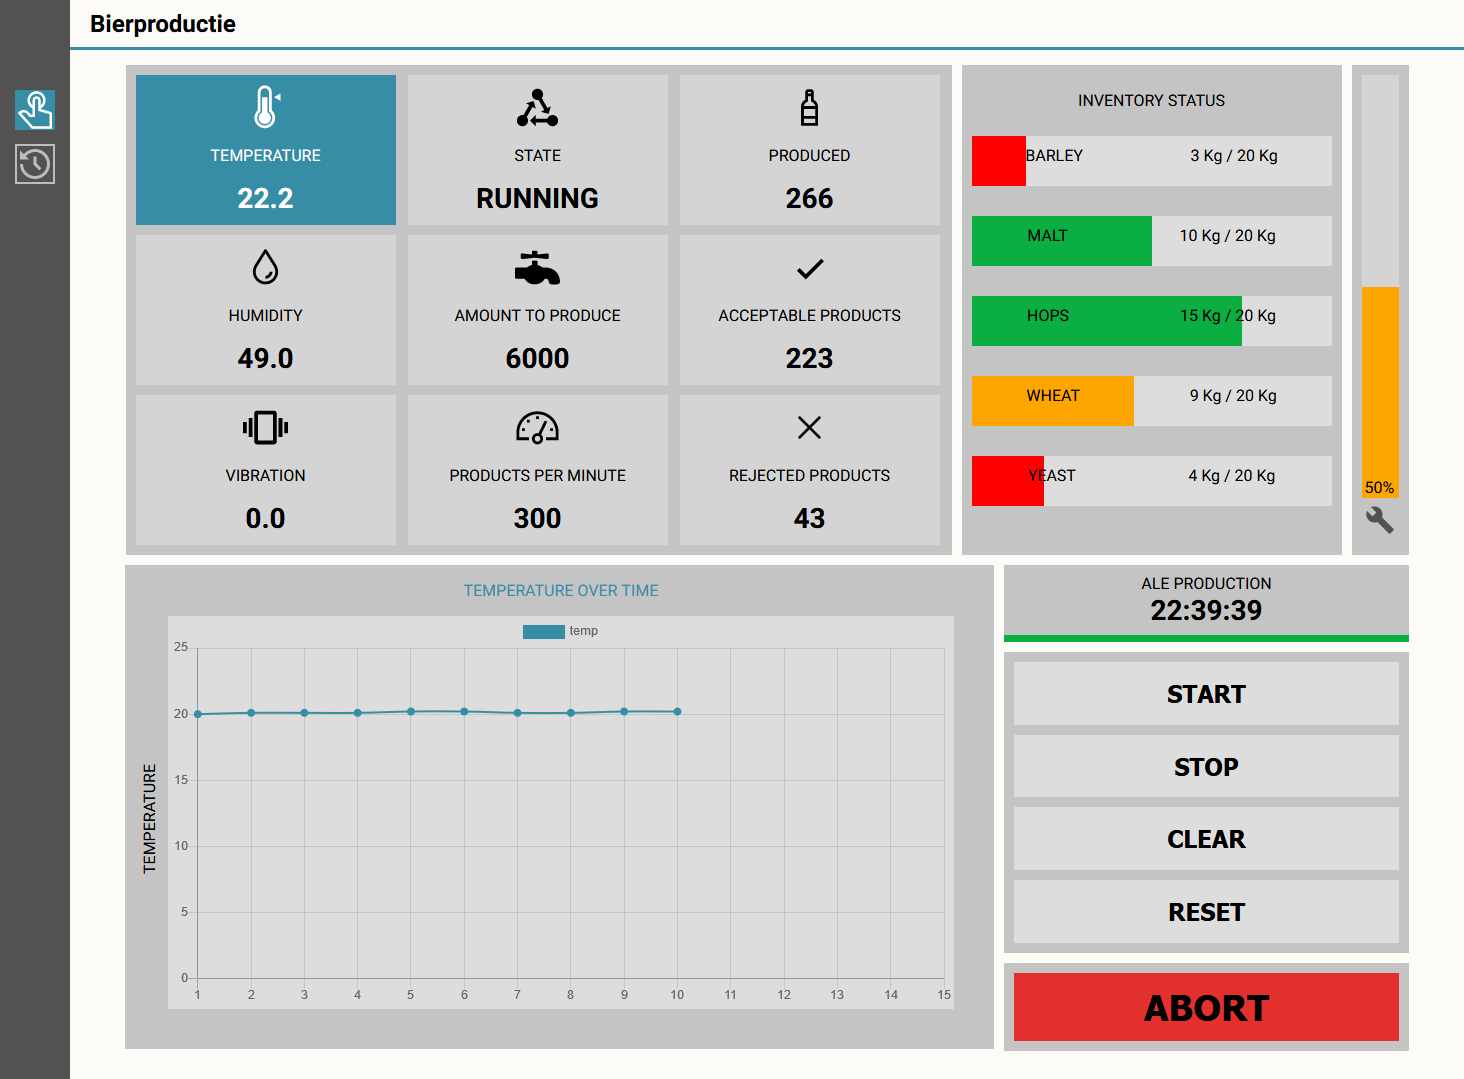
\includegraphics[width=1\linewidth]{images/dashboard.png}
	\caption{Dashboard}
	\label{figure:dashboard}
\end{figure}

The dashboard is implemented using web based technology, so it can run on many
machines without installing any software, apart from a modern browser that is
running JavaScript. It is implemented using HTML, CSS and JavaScript, and it
uses two separate libraries for making graphs and getting icons for the buttons.

\subsection{REST API}

\subsection{Database}

\subsection{OPC-UA-Client}
The OPC-UA-client handles the data from the machine and sends it to the API. It 
is written in Java and uses the Milo library to create a client that connects to 
the machines OPC-UA-server. The OPC-UA-client is able to subscribe to 
information on the server and send it to the API that stores it in the database.
The client also controls the machine while it collects data, as it creates and
runs batches it gets from the dashboard through the API. The client sends live
data to the dashboard via the API using subscriptions. These subscriptions sends
data to the API every time a change appears and the API then forwards it to the
dashboard. The client creates 6 subscriptions when started, they monitor
temperature, vibration, humidity, machine-state,  current defective products and
current processed products. \\

The data is also stored in an object called Batch in the client. The Batch class
has properties corresponding to the values the API uses as well as logic to
process the data. This logic includes OEE calculation and JSON exportation. In
the start of a batch, when the user has configured the desired production, the
data is sent to the client to create a Batch object. The Batch object is then
run with the BatchHandler class, and while the batch is being produced, the
subscriptions will add data to the object. When done the Batch object will run
through its logic and finally export itself as a JSON so it can be sent to the
API. 


\subsection{Overall Equipment Effectiveness}
When a batch is complete, and the data is stored in the batch class, the
calculation of the OEE takes place.\\

The planned production time can not be estimated for this project, as too many
variables are unknown (shift lengths, the time it takes to refill ingredients,
the time it takes to do maintenance work etc.). Therefore, it has been decided
to use the time it takes to produce a batch. The calculation can be seen
below.

\[PlannedProductionTime = \left(\frac{AmountToProduce}{MachineSpeed}\right)\cdot60\]\\

Where the amount to produce divided by the machine speed gives us the production
time in minutes, as the machine speed is products per minute. This result can be
multiplied by 60 to give the production time in seconds. To find the ideal cycle
time the maximum machine speed is needed. 1 divided by this multiplied by 60
then results in the theoretical minimum time it takes to produce one unit.

\[IdealCycleTime = \frac{1}{maxMachineSpeed}\cdot60\]\\

When these have been calculated, it is possible to calculate the OEE using
Equation \ref{eq:OEE}.

\[OEE = \left(\frac{AcceptedProducts\cdot{IdealCycleTime}}{PlannedProductionTime}\right)\cdot100\]\\

This result gives the overall equipment effectiveness in percentage, which is
used to evaluate if the production can be optimised further. It should be noted
that the result from this calculation is only indicative, as neither quality,
performance or availability can be assessed from this.

To give an example on how a calculation with real values would look like, take
the values: amount to produce = 100, maximum machine speed = 300, batch machine
speed = 200, accepted products = 97.

\[PlannedProductionTime = \left(\frac{100}{200}\right)\cdot60 = 30\]

\[IdealCycleTime = \frac{1}{300}\cdot60=0.2\]

\[OEE = \left(\frac{97\cdot0,2}{30}\right)\cdot100 = 64,67\%\]\\

The OEE for this specific batch would be 64,67\%, which means that the
production line can be optimised further if needed.

\subsection{Error Function}
The error function associated with each product type is to be estimated. For
this, several batches should be produced to have some data to do the
calculations with. The variables used to estimate the error function is the
amount of products to produce, the machine speed and the amount of rejected
products. These values are used to make an expression, that resembles the error
function. The data used can be found in Appendix \ref{app:batch_data}.

\begin{figure}[ht]
	\centering
	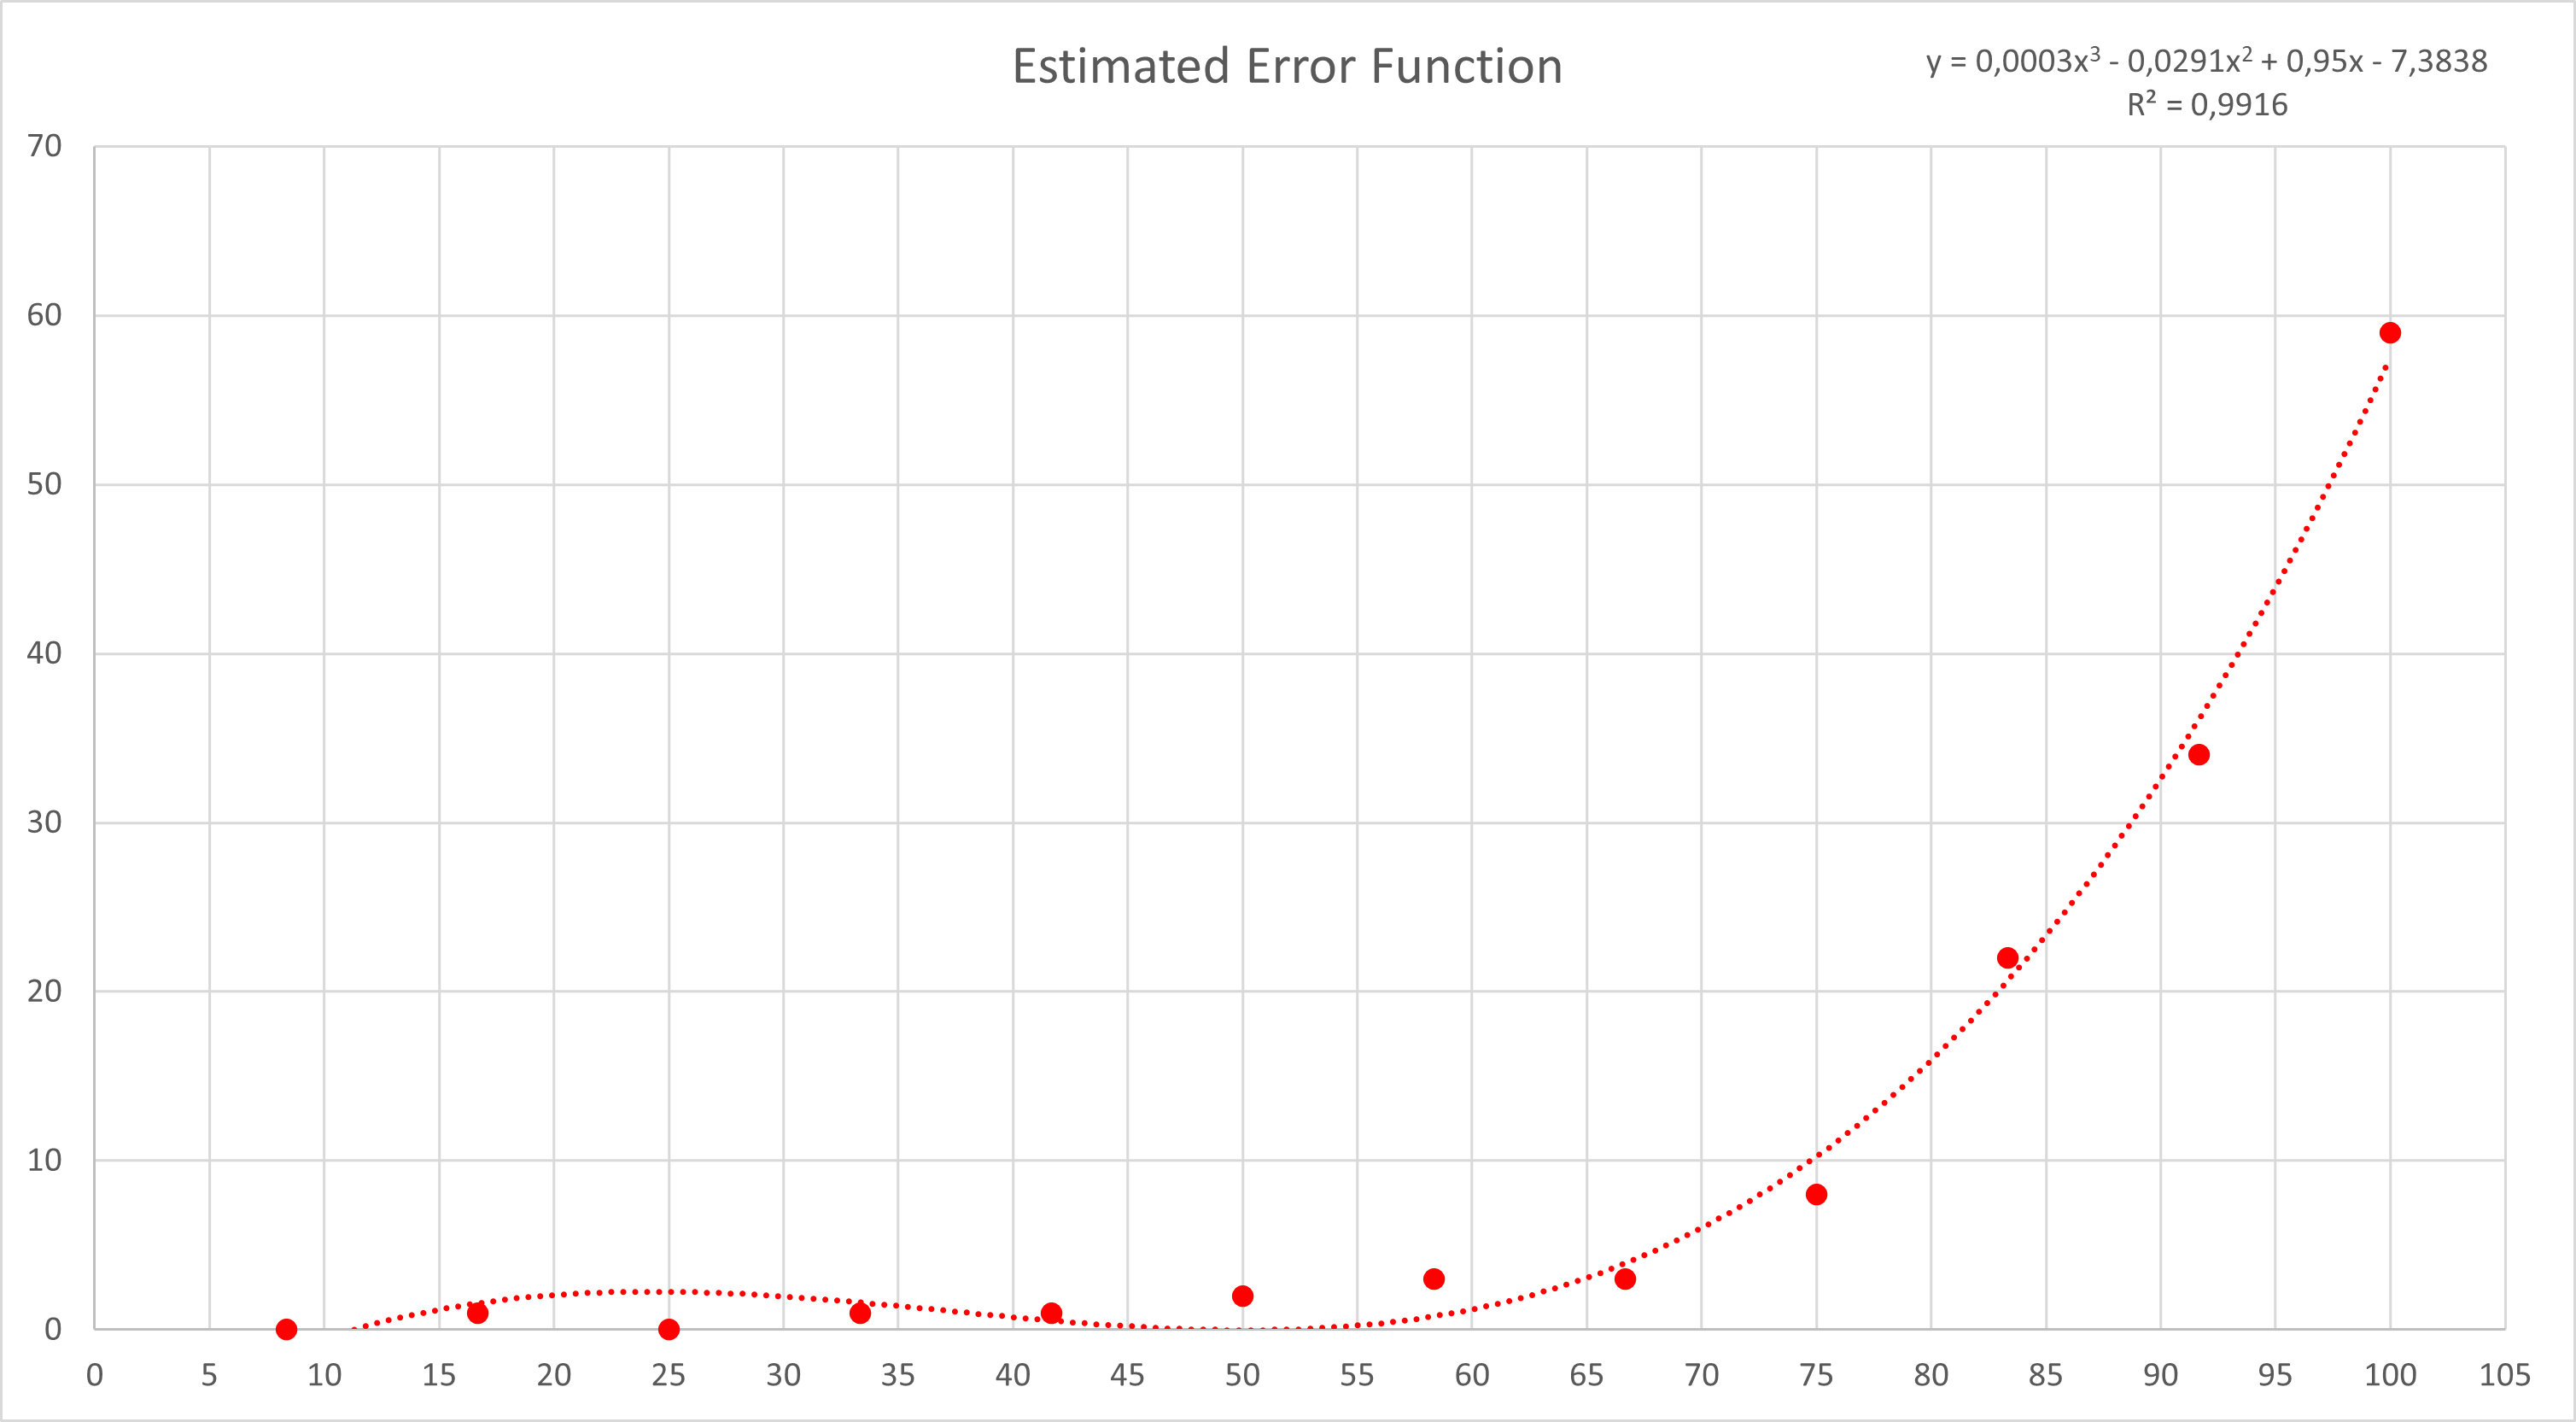
\includegraphics[width=1\linewidth]{images/errorfunction/pilsner.png}
	\caption{Estimated Error Function for Pilsner}
	\label{figure:ef_pilsner}
\end{figure}

The estimated error function seen in Figure \ref{figure:ef_pilsner} gives an
idea of when the beer production machine starts to produce many rejected
products. All the estimated error functions for the products the machine can
produce can be seen in Table \ref{table:eef} and the graphs can be found in
Appendix \ref{app:error_function_graphs}.

\begin{table}[ht]
     \begin{tabularx}{\textwidth}{|>{\RaggedRight}p{3cm}|>{\RaggedRight}X|>{\RaggedRight}p{3cm}|}
     \hline
     \textbf{Product type} & \textbf{Estimated Error Function} & \textbf{Accuracy} \\
     \hline
     Pilsner & \(y = 0,0003x^3 - 0,0291x^2 + 0,95x - 7,3838\) & \(R^2 = 0,9905\) \\
     \hline
     Wheat & \(y = 5E-05x^3 - 0,0077x^2 + 1,3163x - 3,6317\) & \(R^2 = 0,9983\) \\
     \hline
     IPA & \(y = -0,0001x^3 + 0,0548x^2 - 3,7529x + 72\) & \(R^2 = 0,9981\) \\
     \hline
     Stout & \(y = -0,0002x^3 + 0,0319x^2 - 1,551x + 67,071\) & \(R^2 = 0,9331\) \\
     \hline
     Ale & \(y = -2E-05x^3 + 0,0099x^2 - 0,5615x + 9,1857\) & \(R^2 = 1\) \\
     \hline
     Alcohol Free & \(y = 3E-05x^3 - 0,0021x^2 + 0,4464x + 10\) & \(R^2 = 0,9935\) \\
     \hline
    \end{tabularx}
    \caption{Estimated Error Functions}
    \label{table:eef}
\end{table}

\subsection{Optimal Production Speed}
To find the optimal production speed, the same data as when estimating the error
function is used. As the error simulation in the machine is a function of the
normalised machine speed and the selected product, the normalised machine speed
must be calculated. This is done by taking 100 over the maximum machine speed.
This, multiplied by the chosen machine speed will then give the percentage of
the maximum machine speed, which is used when plotting the graph for the optimal
production speed. The normalised machine speed will be the \(x\)-values and the
calculated OEE will be the \(y\)-values. An example can be seen in Figure
\ref{figure:ops_pilsner}, where the graph for the optimal production speed for
the product type pilsner can be seen.

\begin{figure}[ht]
	\centering
	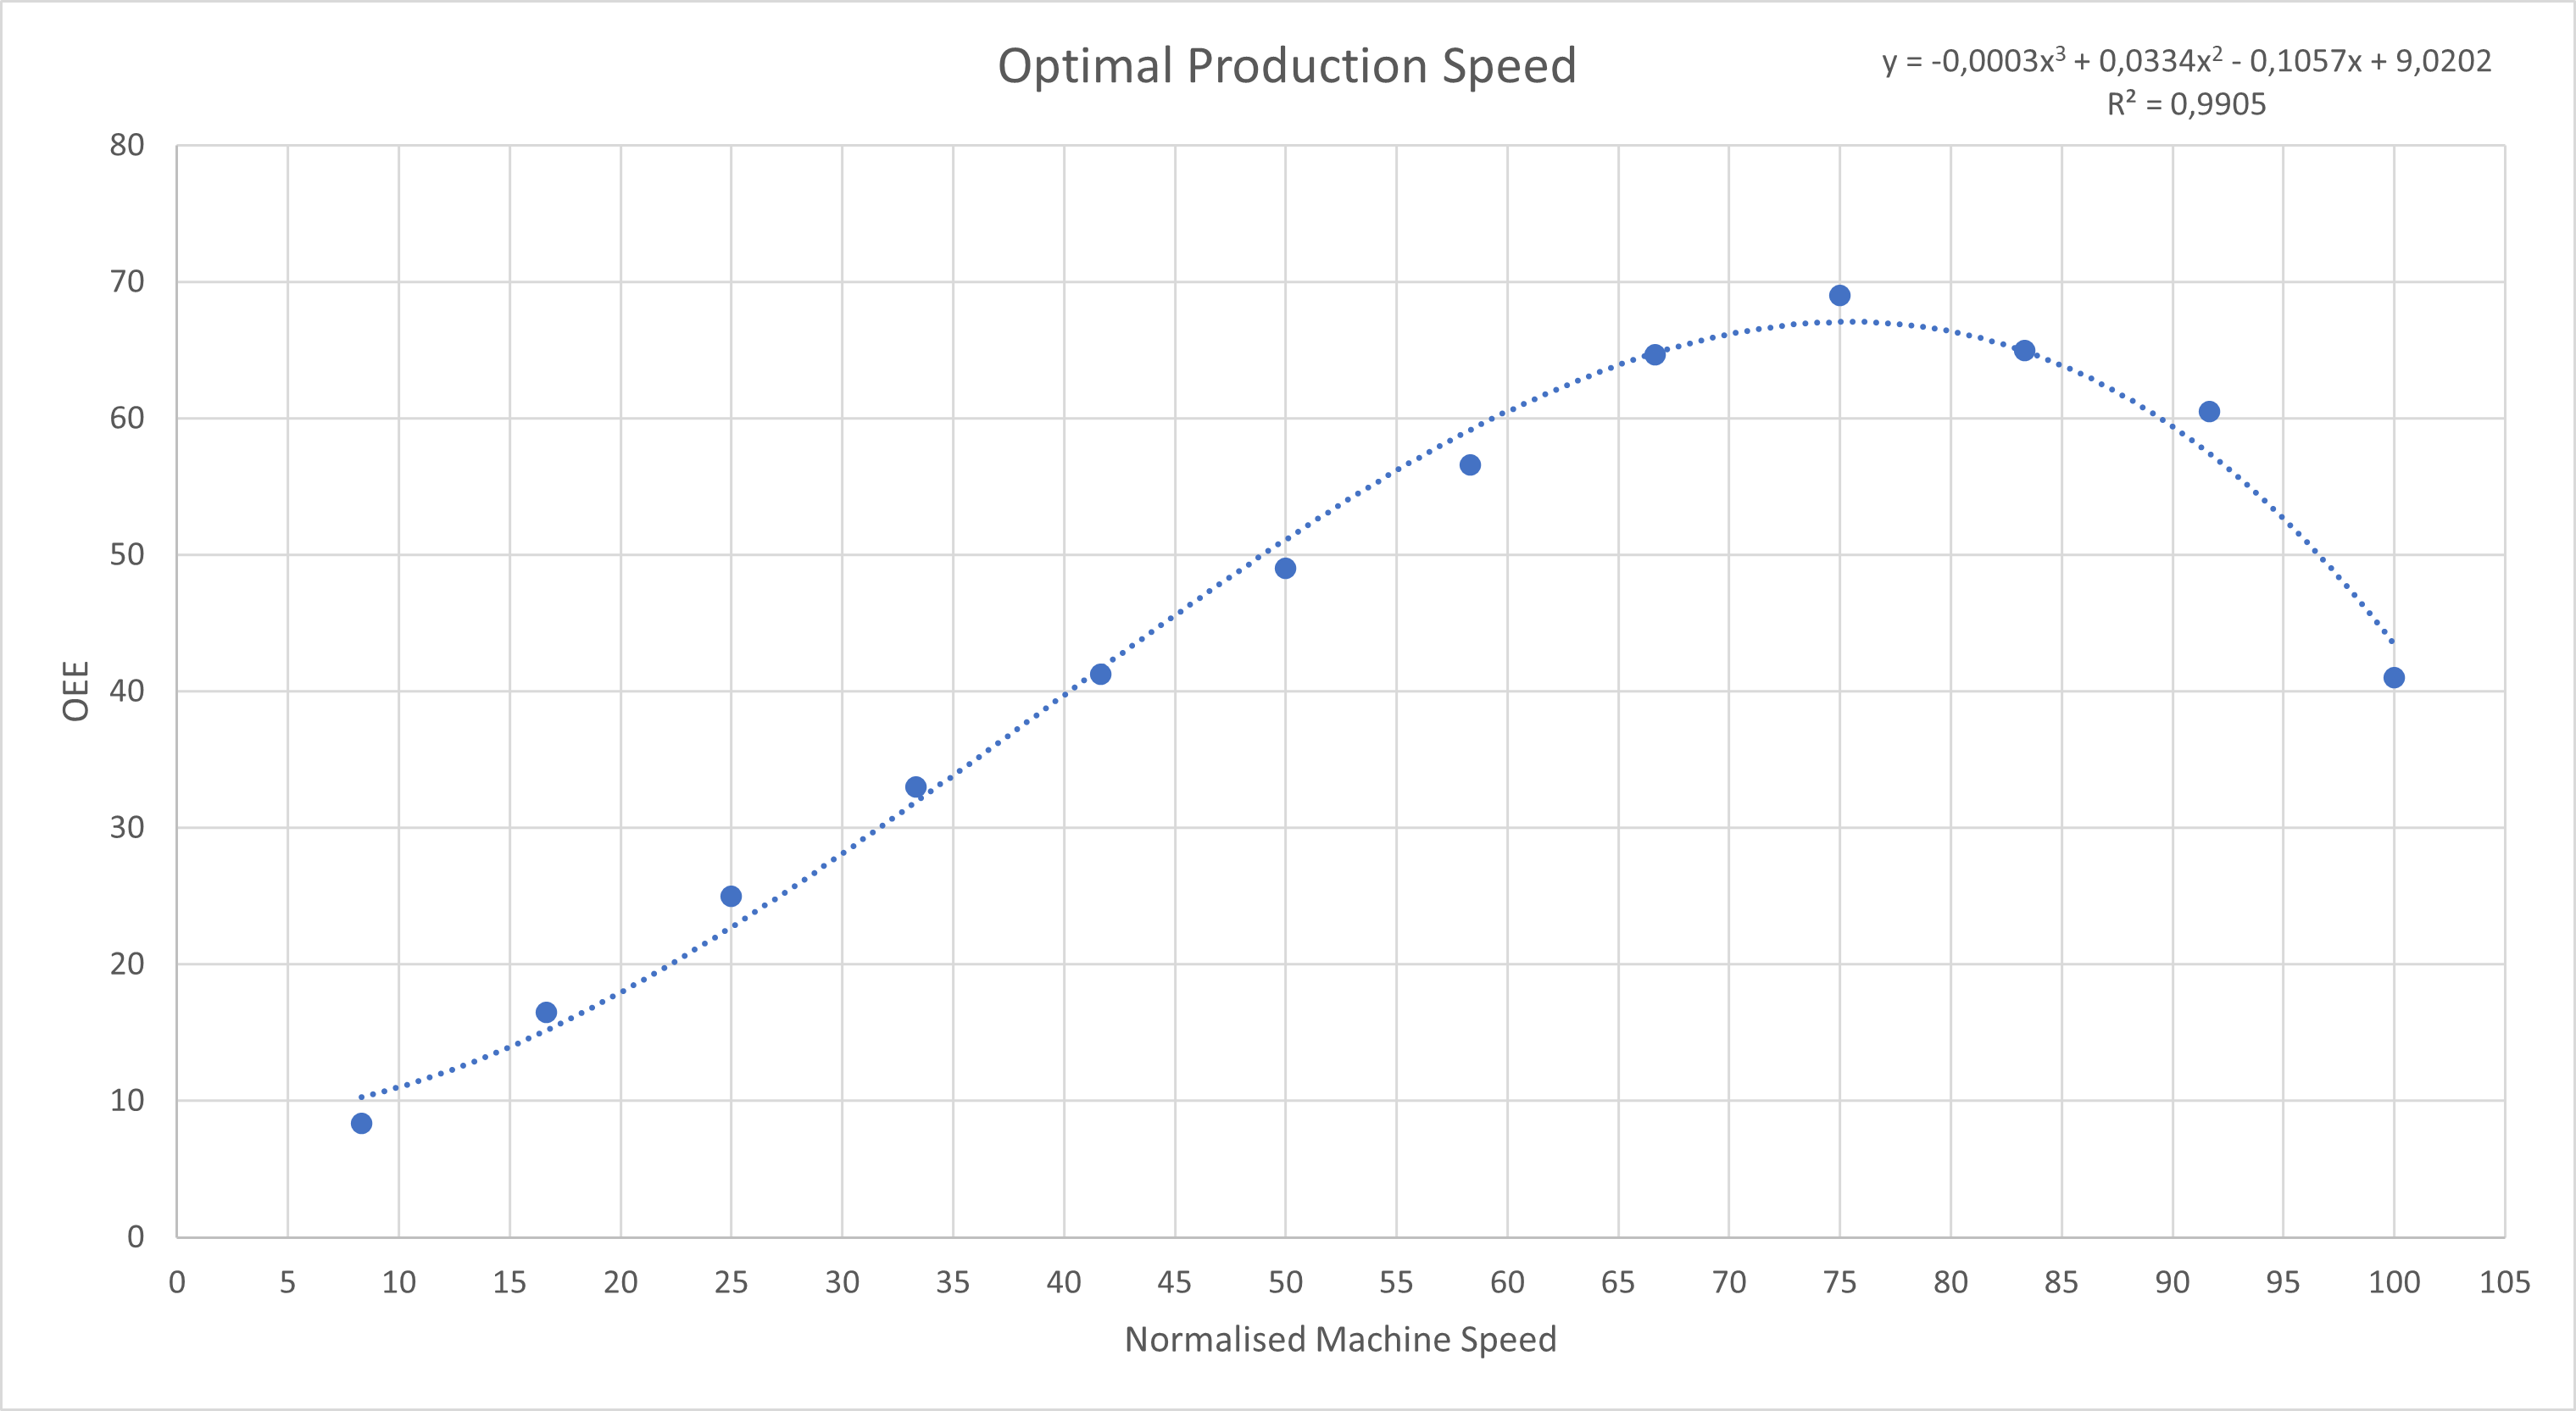
\includegraphics[width=1\linewidth]{images/ops/pilsner.png}
	\caption{Optimal Production Speed for Pilsner}
	\label{figure:ops_pilsner}
\end{figure}

This plot is generated using Microsoft Excel. When the OEE for each tested
machine speed is plotted, a third-degree polynomial trend line is applied and an
expression for the function generated is given. For the pilsner, the function is
given by:

\[y = -0,0003x^3+0,0334x^2-0,1057x+9,0202\]


With an \(R^2\) of \(0,9905\) which is used to see how close to the data points
the polynomial is (the closer to 1 the more accurate).\\

To find the maximum of the function, the derivative is calculated:

\[y' = -\frac{9x^2-668x+1057}{10000}\]

To find the maximum this equation should be solved for \(x\) when \(y=0\). This
gives \(72,61\), which is the optimal machine speed for the pilsner product type,
measured in percentage of the maximum machine speed.

To make sure the calculated \(x\)-value is a local maximum at \(72,61\),
the second derivative is calculated:

\[y'' = -\frac{18x-668}{10000}\]

Then, this equation is solved for \(y\) when \(x=72,61\), which gives a value of
\(-0,06\). Since the result is less than 0, it can be confirmed that it is
a maximum.\\

This is done for all product types, and the result can be seen in Table
\ref{table:ops}.


\begin{table}[ht]
     \begin{tabularx}{\textwidth}{|>{\RaggedRight}p{3cm}|>{\RaggedRight}X|>{\RaggedRight}p{6cm}|}
     \hline
     \textbf{Product type} & \textbf{Maximum} & \textbf{Optimal Production Speed}\\
     \hline
     Pilsner & 72,61\% of 600 & 435,63 products/minute \\
     \hline
     Wheat & 51,58\% of 300 & 154,75 products/minute \\
     \hline
     IPA & 62,55\% of 150 & 93,83 products/minute \\
     \hline
     Stout & The equation has no solution for \(x\) in ${\rm I\!R}$ & 200 products/minute (max) \\
     \hline
     Ale & 91,82\% of 100 & 91,82 products/minute \\
     \hline
     Alcohol Free & 76,35\% of 125 & 95,44 products/minute \\
     \hline
    \end{tabularx}
    \caption{Optimal Production Speed}
    \label{table:ops}
\end{table}


The reason for the result of the stout is that the function has no local maxima
in the range (0 to 200). Instead, it keeps increasing, as seen in the graph for the
stout in Appendix \ref{app:ops_graphs}. This means that the faster the machine speed
the better, which is why the optimal production speed is the maximal machine
speed.
